\documentclass{article}
\usepackage{graphicx}
\usepackage[utf8]{inputenc}
\usepackage[OT1]{fontenc}
\usepackage{subcaption}
\usepackage{babel}

\begin{document}

\title{Introduction and Course Overview}
\author{Felipe Glicério Gomes Marcelino}
\date{18 April 2020}
\maketitle

\section{Notes}

\subsection*{Slide 11}
\par Reinforcement learning is an excellent method  build intelligent machines.

\subsection*{Slide 12}
\par Some intelligent machines to imitate human behavior is challenging to develop. It is because humans are not just
smart, but they are good at solving problems and they are highly adaptable.

\subsection*{Slide 13}
\par Deep learning is very good at handling unstructured because they can learn from large amounts of data and
discover patterns.

\subsection*{Slide 14}

\par Reinforcement learning provides a formalism for behavior. It is a mathematical formalization of a decision-making problem. Reinforcement learning has an agent,
an environment, and the agent interacts with the environment creating an action for a specific state of the environment. Subsequently, the environment returns a response taking into account the action.

\par Reinforcement learning has an essential role in tasks like playing games. The success of reinforcement learning
is the capacity to defeat your opponent.


\subsection*{Slide 15}
\par 
Deep reinforcement learning removes the need to extract features manually. For example, using CNN as a policy, it is only necessary to pre-process the image and pass this through the model. The model going to learn how to
extract the features correctly using the outcome generated by action to update


\subsection*{Slide 21}

\begin{figure}
    \centering
    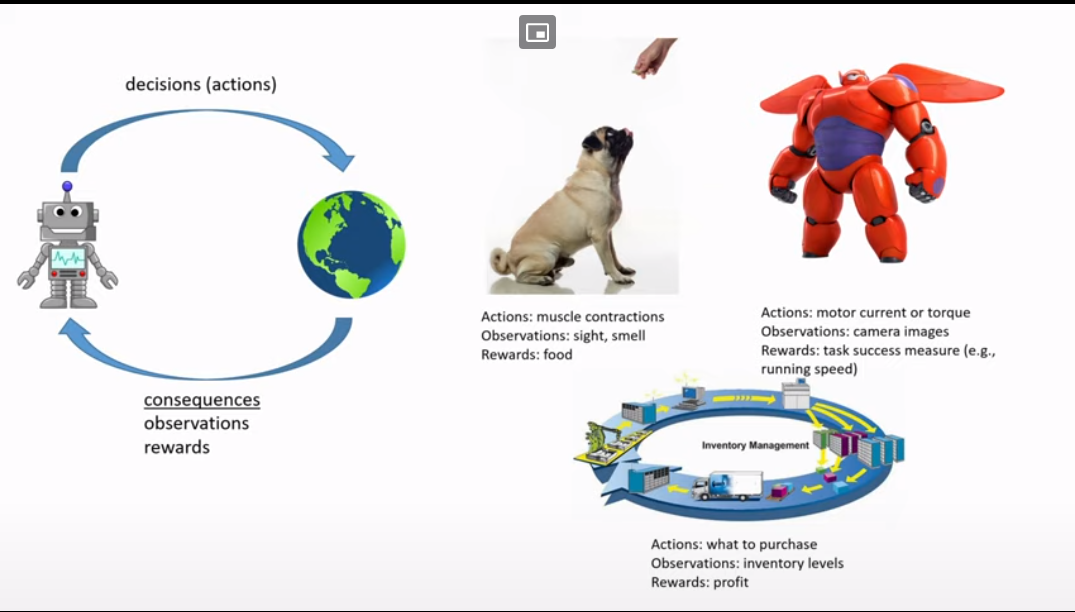
\includegraphics[scale=0.4]{cap1img/slide21.png}
    \caption{Framework of reinforcement learning}
    \label{fig:slide21}
\end{figure}

\par Figure \ref{fig:slide21} shows how the framework of reinforcement learning works. It has three elements:
\begin{itemize}
    \item Agent: Responsible to make an action using the observation space
    \item Observation Space: Data used to assist the agent
    \item Reward: Consequence of the action made by the agent
\end{itemize}

\subsection*{Slide 27}
\par Why should we study deep reinforcement learning this now?
\begin{enumerate}
    \item  Advances in deep learning - We can create complex architecture networks and training them using
        sophisticated techniques to understand  high dimensional observation spaces, such as images.
    \item  Advances in reinforcement learning - We have algorithms with favorable numerical properties, they are
        stable to use and reliable. It can converge to reasonable solutions.
    \item Advances in computational capability - More power to process, more advanced tasks the model can realize.
\end{enumerate}

\subsection*{Slide 31}%
\label{sub:Slide 31}

\par 
\begin{enumerate}
    \item Basic reinforcement learning deals with maximizing rewards
    \item Inverse reinforcement learning - Learning reward functions from examples
    \item Transferring knowledge between domains (transfer learning, meta-learning)
    \item Learning to predict and using prediction to act
\end{enumerate}

\subsection*{Slide 42}%
\label{sub:Slide 42}
\par How do we build intelligent machines? It is possible to program and execute in a computer imitation of the brain.  However, each of these parts from the brain is quite complicated to emulate.

\par With this in mind, the idea behind reinforcement learning is implementing learning algorithms and creating machines 
capable of executing simple and complex tasks.


\subsection*{Slide 46}%
\label{sub:Slide 46}
\par 
Algorithms used by deep reinforcement learning field must be capable of interpreting rich sensory inputs, as images,
and choose complex actions. Consequently, it is necessary to use deep learning as base algorithms. Deep = can process
complex.


\end{document}
